\chapter{Laboratorio 4: \\Bus Encoding}
Durante questa esperienza di laboratorio, viene chiesto di analizzare e di valutare alcune tecniche di bus encoding. Nella prima parte dell'esperienza viene chiesto di valutare le performance delle varie tecniche in termini di transizioni e poi sintetizzare il sistema e verificare il consumo di potenza
\section{Simulation}
Durante la prima parte dell'esperienza viene chiesto di valutare, in termini di commutazioni, diverse tecniche di bus-encoding. Il tutto viene simulato grazie ad un testbench fornito e tramite i \textit{power report} generati da \textit{ModelSim}.
\subsection{Non-encoded}
Inizialmente si è simulato il caso in cui utilizzi un bus non codificato, andando a vedere l'evoluzione dei toogle in 10000 colpi di clock in modo tale da avere un punto di riferimento nel confronto con le altre varie tecniche. All'interno del testbench da simulare sono distinti due processi:
\begin{itemize}
	\item processo per gli indirizzi
	\item processo per i dati
\end{itemize}
i quali prendono come input i dati contenuti nel file \textit{rndin.txt} che, come sottolineato nella traccia, contiene delle stringe da 8 bit con una bassa probabilità di 1 logico. Questo fa già prevedere che la tecnica \textit{Transition-Based} risulterà più performante, in quanto questa tipologia di codifica porta ad una riduzione delle commutazioni, solo nel caso in cui le probabilità di '1' logico e di '0' logico siano fortemente non equiprobabili.
Nelle Figure \ref{report_address_41} e \ref{report_dati_41}, sono riportati i \textit{power report} rispettivamente nel caso di dati e di indirizzi. Infine, nelle Tabelle \ref{Tab1} e \ref{Tab2} si riportano le switching activities rispettivamente nel caso di indirizzi e dati.
\begin{figure}[!htb]
	\centering
	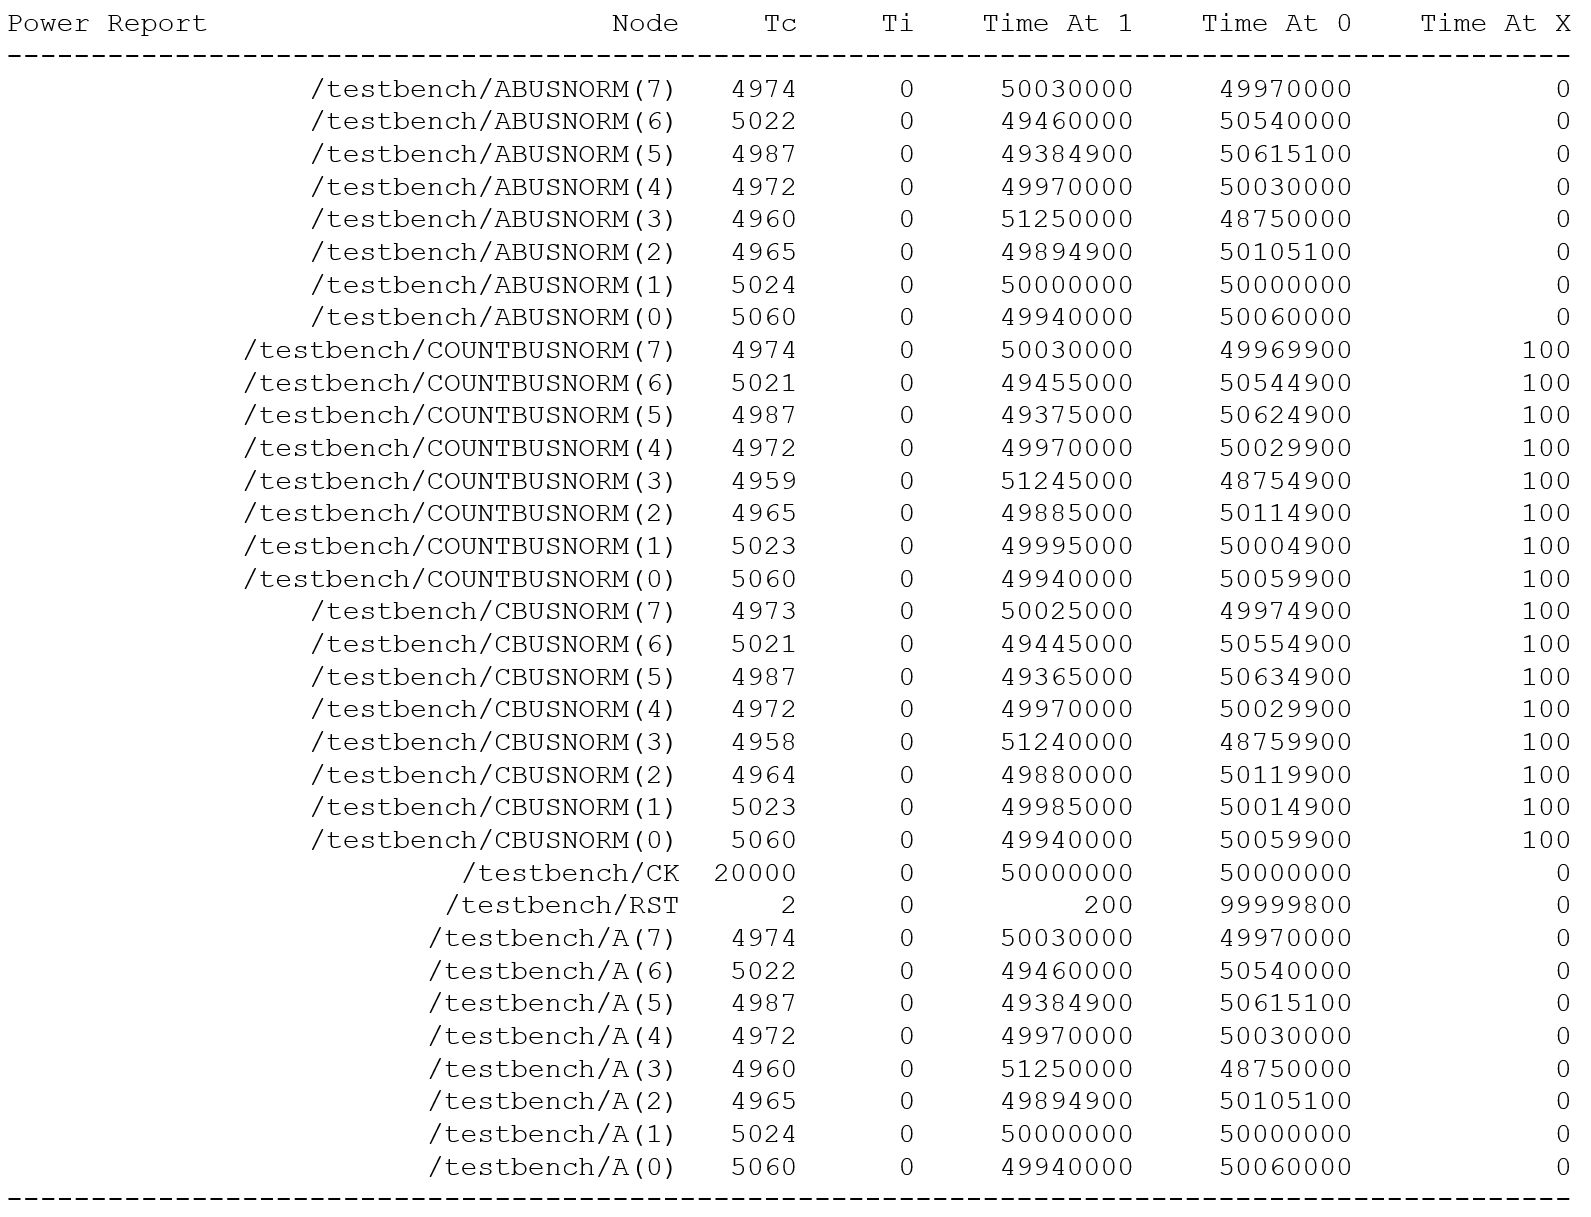
\includegraphics[scale=0.65]{immagini/4_1_data_report}
	\caption{\textit{Power Report, tecnica no-encoding, caso 'data'}}
	\label{report_dati_41}
\end{figure}
\begin{table}[!h]\footnotesize
	\centering
	\begin{tabular}{|c|c|}
		\hline
		\textbf{Nodo} & \textbf{$E_{SW}$}\\
		\hline
		countbusnorm(7) & 0.0097\\
		countbusnorm(6) & 0.0118\\
		countbusnorm(5) & 0.0312\\
		countbusnorm(4) & 0.0624\\
		countbusnorm(3) & 0.1249\\
		countbusnorm(2) & 0.2499\\
		countbusnorm(1) & 0.4999\\
		countbusnorm(0) & 0.9999\\
		\hline
	\end{tabular}
	\caption{\textit{Switching Activity, tecnica no-encoding, caso 'data'}}
	\label{Tab1}
\end{table}
\newpage
\begin{figure}[!htb]
	\centering
	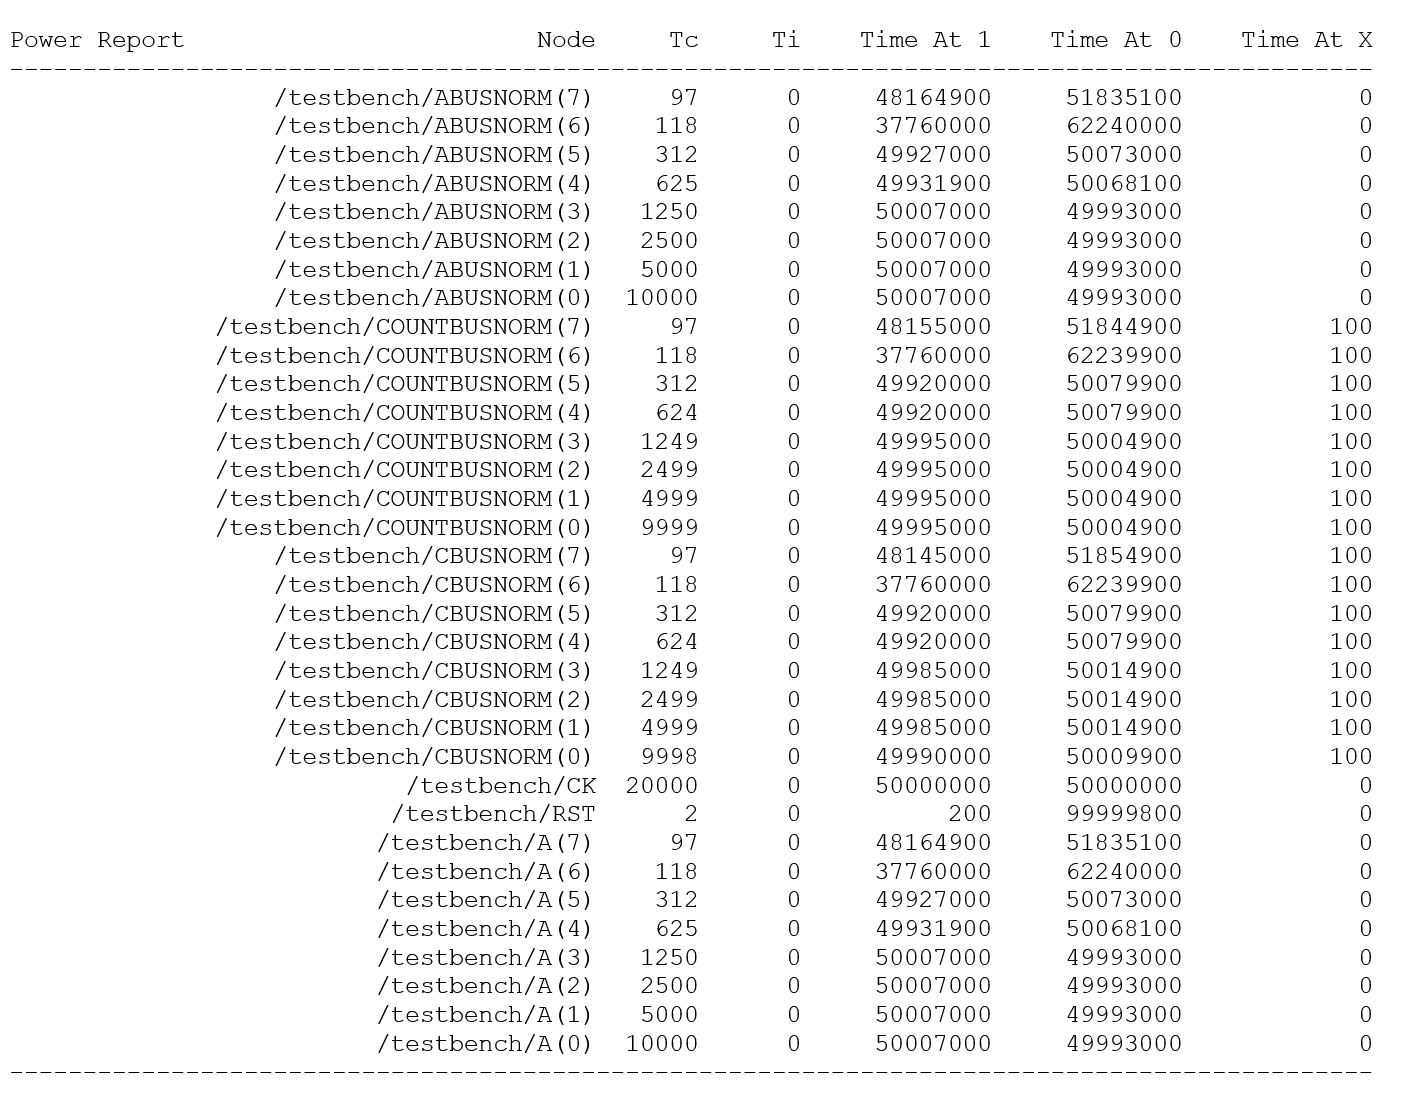
\includegraphics[scale=0.8]{immagini/4_1_addres_report}
	\caption{\textit{Power Report, tecnica no-encoding, caso 'address'}}
	\label{report_address_41}
\end{figure}
\begin{table}[!h]\footnotesize
	\centering
	\begin{tabular}{|c|c|}
		\hline
		\textbf{Nodo} & \textbf{$E_{SW}$}\\
		\hline
		countbusnorm(7) & 0.4974\\
		countbusnorm(6) & 0.5021\\
		countbusnorm(5) & 0.4987\\
		countbusnorm(4) & 0.4972\\
		countbusnorm(3) & 0.4959\\
		countbusnorm(2) & 0.4965\\
		countbusnorm(1) & 0.5023\\
		countbusnorm(0) & 0.506\\
		\hline
	\end{tabular}
	\caption{\textit{Switching Activity, tecnica no-encoding, caso 'address'}}
	\label{Tab2}
\end{table}
\subsection{Bus-invert technique, Transition based technique, Gray technique}
La codifica del Bus-invert consiste nel verificare che il dato successivo comporti un numero di commutazioni superiori di $\frac{N}{2}$, dove N è il numero di linee che compone il bus. In caso, conviene mandare il dato complementato e forzare ad '1' un bit denominato \textit{inv}, per segnalare che il dato in arrivo è in realtà complementato. Nelle Tabelle \ref{Tab3} e \ref{Tab4}, si riportano le Switching Activity rispettivamente nel caso di indirizzi e dati.\\
\begin{table}[!h]\footnotesize
	\centering
	\begin{tabular}{|c|c|}
		\hline
		\textbf{Nodo} & \textbf{$E_{SW}$}\\
		\hline
		countbusinv(8) & 0.0624\\
		countbusinv(7) & 0.0527\\
		countbusinv(6) & 0.0506\\
		countbusinv(5) & 0.0312\\
		countbusinv(4) & 0\\
		countbusinv(3) & 0.0625\\
		countbusinv(2) & 0.1875\\
		countbusinv(1) & 0.4375\\
		countbusinv(0) & 0.9375\\
		\hline
	\end{tabular}
	\caption{\textit{Switching Activity, tecnica bus-invert, caso 'address'}}
	\label{Tab3}
\end{table}
\begin{table}[!h]\footnotesize
	\centering
	\begin{tabular}{|c|c|}
		\hline
		\textbf{Nodo} & \textbf{$E_{SW}$}\\
		\hline
		countbusinv(8) & 0.365\\
		countbusinv(7) & 0.3576\\
		countbusinv(6) & 0.3611\\
		countbusinv(5) & 0.3617\\
		countbusinv(4) & 0.364\\
		countbusinv(3) & 0.3613\\
		countbusinv(2) & 0.3601\\
		countbusinv(1) & 0.3639\\
		countbusinv(0) & 0.3722\\
		\hline
	\end{tabular}
	\caption{\textit{Switching Activity, tecnica bus-invert, caso 'data'}}
	\label{Tab4}
\end{table}

\begin{figure}[!htb]
	\centering
	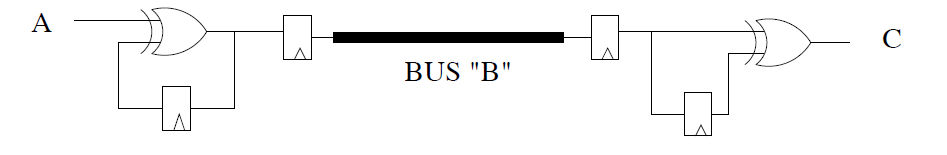
\includegraphics[scale=1.2]{immagini/transition}
	\caption{\textit{Schema tecnica 'Transition Based'}}
	\label{transition}
\end{figure}
\noindent Si esegue la medesima analisi per la tecnica \textit{Transition Based}, riportata in Figura \ref{transition}. Questa tecnica consiste nell'inviare uno '0' logico ogni qual volta la linea corrisponde alla precedente, mentre un '1' logico viene inteso come complemento del valore precedente della linea. I risultati delle simulazioni sono riportati per il caso dati in Tabella \ref{Tab5} e per il caso indirizzi in Tabella \ref{Tab6}. \\
\begin{table}[!h]\footnotesize
	\centering
	\begin{tabular}{|c|c|}
		\hline
		\textbf{Nodo} & \textbf{$E_{SW}$}\\
		\hline
		countbustran(7) & 0.5003\\
		countbustran(6) & 0.4946\\
		countbustran(5) & 0.4938\\
		countbustran(4) & 0.4997\\
		countbustran(3) & 0.5125\\
		countbustran(2) & 0.4989\\
		countbustran(1) & 0.500\\
		countbustran(0) & 0.4994\\
		\hline
	\end{tabular}
	\caption{\textit{Switching Activity, tecnica Transition-Based, caso 'data'}}
	\label{Tab5}
\end{table}
\begin{table}[!h]\footnotesize
	\centering
	\begin{tabular}{|c|c|}
		\hline
		\textbf{Nodo} & \textbf{$E_{SW}$}\\
		\hline
		countbustran(7) & 0.4816\\
		countbustran(6) & 0.3776\\
		countbustran(5) & 0.4992\\
		countbustran(4) & 0.4992\\
		countbustran(3) & 0.500\\
		countbustran(2) & 0.500\\
		countbustran(1) & 0.500\\
		countbustran(0) & 0.500\\
		\hline
	\end{tabular}
	\caption{\textit{Switching Activity, tecnica Transition-Based, caso 'address'}}
	\label{Tab6}
\end{table}
\begin{figure}[!htb]
	\centering
	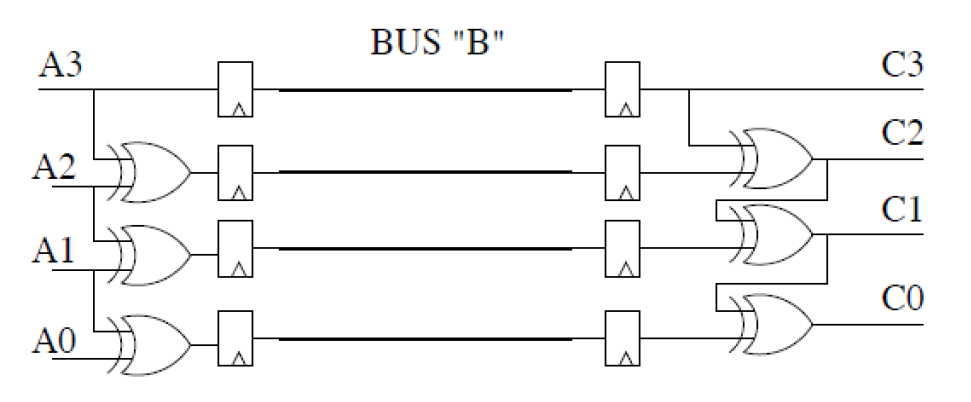
\includegraphics[scale=1]{immagini/gray}
	\caption{\textit{Schema tecnica 'Codifica di Gray'}}
	\label{gray}
\end{figure}
\newpage
\noindent La tecnica \textit{Codifica di Gray}, riportata in Figura \ref{gray}: questa tecnica viene sfruttata specialmente nelle trasmissioni sequenziali, come ad esempio nel caso di indirizzi, in modo tale da cambiare esclusivamente un solo bit alla volta. I risultati delle Switching Activities sono riportati per i dati nella Tabella \ref{Tab7} e nella Tabella \ref{Tab8} per gli indirizzi. \\
\begin{table}[!h]\footnotesize
	\centering
	\begin{tabular}{|c|c|}
		\hline
		\textbf{Nodo} & \textbf{$E_{SW}$}\\
		\hline
		countbusgray(7) & 0.4974\\
		countbusgray(6) & 0.5087\\
		countbusgray(5) & 0.4952\\
		countbusgray(4) & 0.4981\\
		countbusgray(3) & 0.4937\\
		countbusgray(2) & 0.5056\\
		countbusgray(1) & 0.4962\\
		countbusgray(0) & 0.5075\\
		\hline
	\end{tabular}
	\caption{\textit{Switching Activity, tecnica Codifica di Gray, caso 'data'}}
	\label{Tab7}
\end{table}
\begin{table}[!h]\footnotesize
	\centering
	\begin{tabular}{|c|c|}
		\hline
		\textbf{Nodo} & \textbf{$E_{SW}$}\\
		\hline
		countbusgray(7) & 0.097\\
		countbusgray(6) & 0.055\\
		countbusgray(5) & 0.194\\
		countbusgray(4) & 0.312\\
		countbusgray(3) & 0.625\\
		countbusgray(2) & 0.125\\
		countbusgray(1) & 0.250\\
		countbusgray(0) & 0.500\\
		\hline
	\end{tabular}
	\caption{\textit{Switching Activity, tecnica Codifica di Gray, caso 'address'}}
	\label{Tab8}
\end{table}
\newpage
\noindent Si riportano per completezza i \textit{Power Report} delle simulazioni svolte con \textit{ModelSim}. In Figura \ref{address} si riporta il Report nel caso di indirizzi, mentre in Figura \ref{data} il caso di dati.
\\
\\
\begin{figure}[!htb]
	\centering
	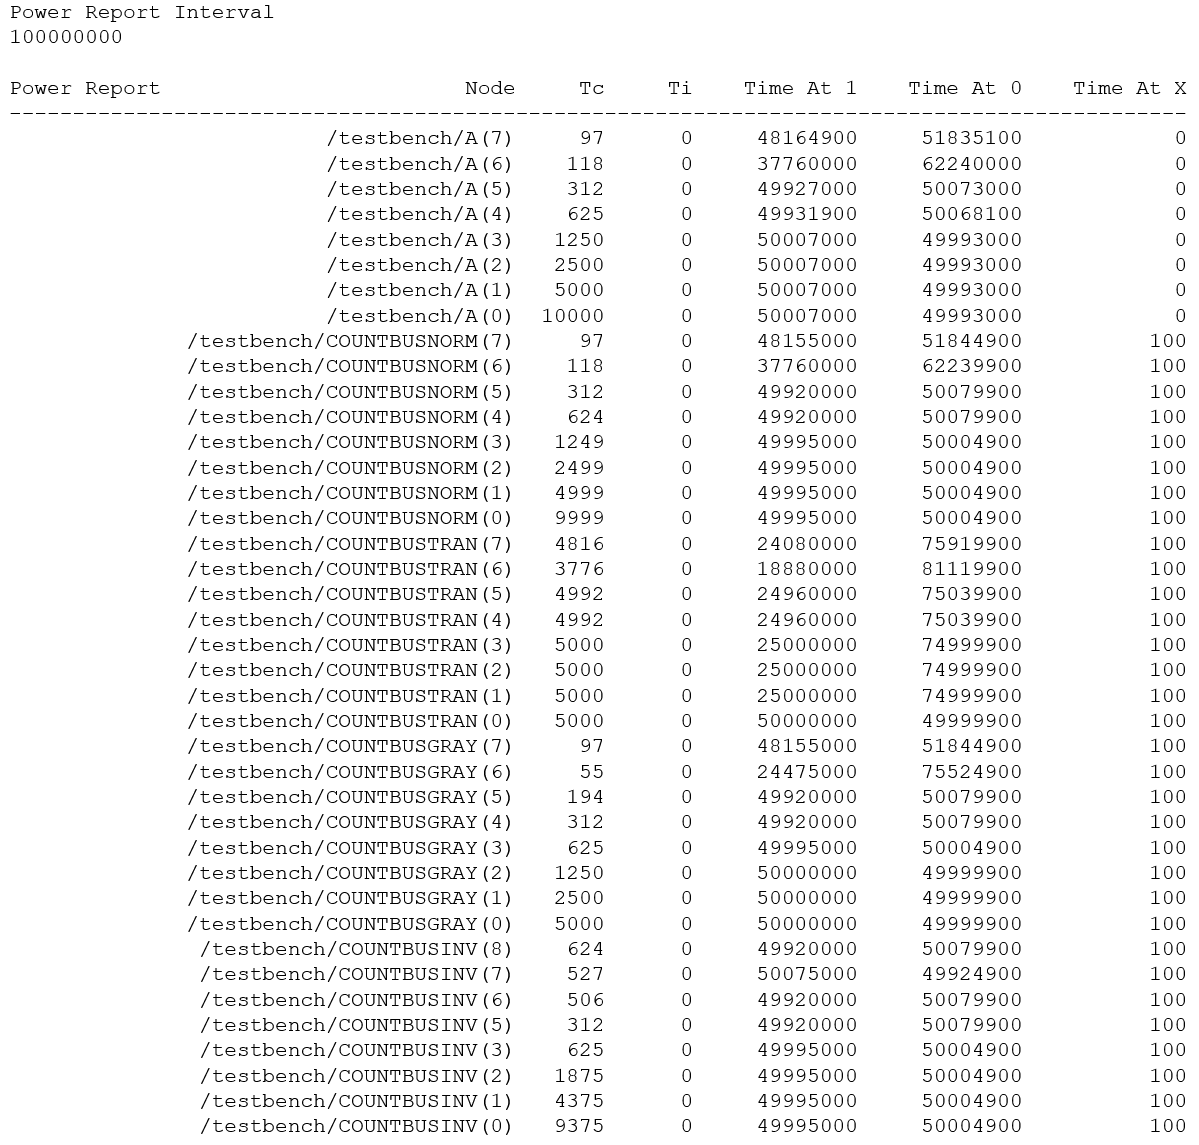
\includegraphics[scale=1]{immagini/address_report_tecniche}
	\caption{\textit{Power Report complessivo, caso 'address'}}
	\label{address}
\end{figure}
\newpage
\begin{figure}[!htb]
	\centering
	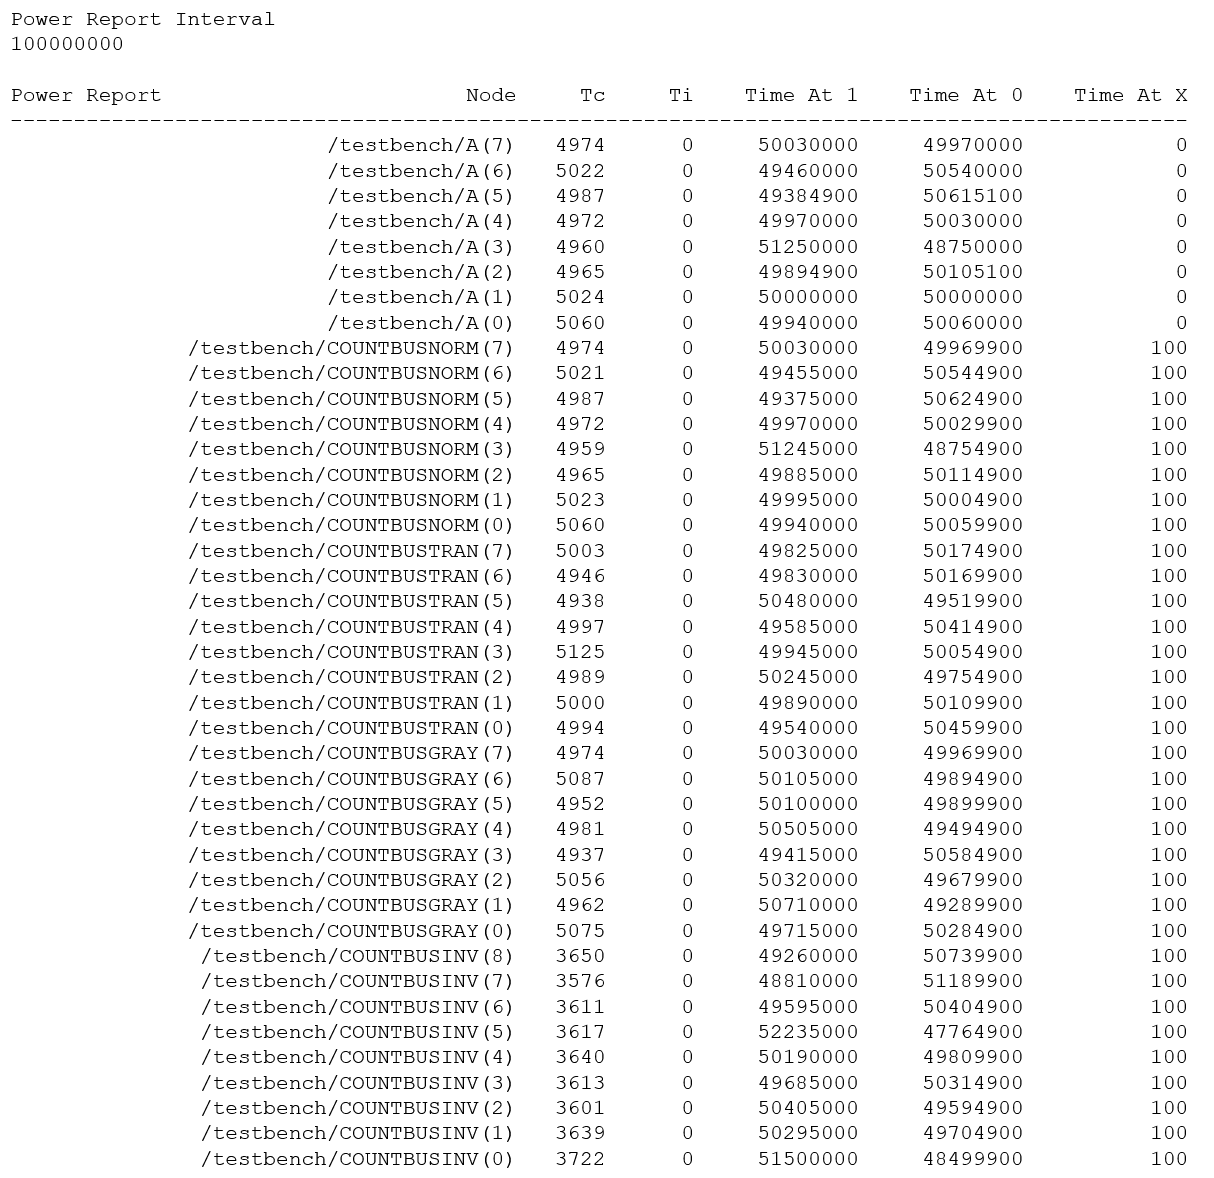
\includegraphics[scale=0.8]{immagini/data_report_tecniche}
	\caption{\textit{Power Report complessivo, caso 'data'}}
	\label{data}
\end{figure}
\subsection{T0 techinque}
L'ultima tecnica richiesta è di implementare un codice per realizzare la tecnica \textit{T0 Encoding}. Nella traccia viene riportata la formula richiesta da implementare, riportata anche in Figura \ref{formula_t0}.\\
\begin{figure}[!htb]
	\centering
	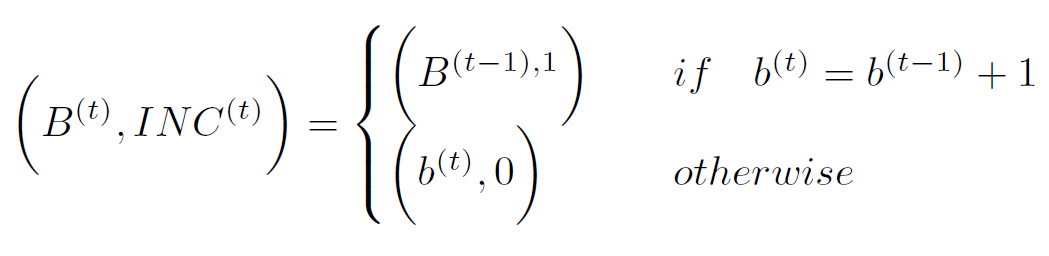
\includegraphics[scale=0.8]{immagini/formula_t0}
	\caption{\textit{Formula implementata, tecnica 'T0'}}
	\label{formula_t0}
\end{figure}
\\
\noindent La codifica T0 consiste nell'inserire un bit in più, denominato \textit{INC}. Ogni volta che si va in sequenza, si forza questo segnale a '0' in modo tale che il ricevitore capisca di dover andare semplicemente in sequenza e si preoccupi lui di incrementare il dato. In caso di brach, salito o subroutine, forzo il segnale ad '1' e trasmetto sul bus il nuovo dato. Si riporta in appendice fig. \ref{t0} il \textit{Codice VHDL} dell'implementazione della codifica.
Sono state effettuate con modelsim le simulazioni di consumo di potenza e riportate di seguito rispettivamente per address fig   e data fig. . 
\begin{figure}[!htb]
	\centering
	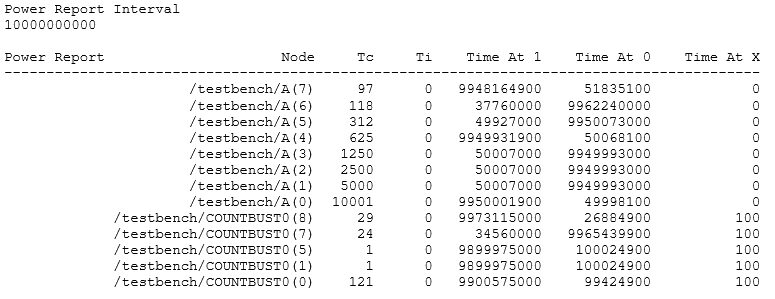
\includegraphics[scale=0.8]{immagini/T0_address_power}
	\caption{\textit{Power report T0, address}}
	\label{T0_address_power}
\end{figure}
\begin{figure}[!htb]
	\centering
	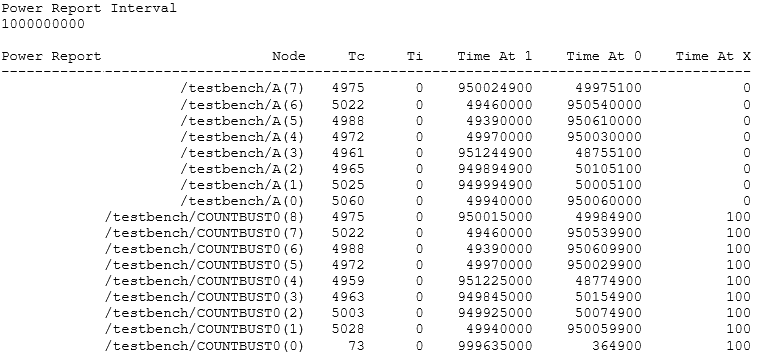
\includegraphics[scale=0.8]{immagini/T0_data_power}
	\caption{\textit{Power report T0, data}}
	\label{T0_data_power}
\end{figure}
\subsection{Confronto tra le tecniche}
Confrontando i risultati tra le varie tecniche, si può notare come l'unica tecnica che porta ad una riduzione dei consumi nel caso dei dati, risulta essere la \textbf{Bus-Invert} con la quale si ottiene un risparmio sulle commutazioni pari a circa il 20\%. \\ %DATO DA VERIFICARE
Per quanto concerne la tramissione di indirizzi, le codifiche più perfomanti risultano la \textbf{Codifica di Gray}, che porta ad un risparmio sulle commutazioni del 50\%, e la \textbf{Codifica T0}, che porta ad un risparmio del XX\%.\\
Si può notare come la tecnica che risulta meno performante è la \textbf{Transition Based}, che porta ad un incremento del 93\% nel caso di dati e ad un incremento circa del 0,1\% nel caso di indirizzi. Ovviamente questo è concorde con quanto ci si aspettava, in quanto, come già detto prima, questa tipologia di decofica funziona efficentemente solo nel caso in cui le probabilità di '1' e di '0' logico non risultino sbilanciate.

\section{Synthesis}
Una volta aver stimato il consumo di potenza per la tecnica di bus non-encoded si può adesso calcolare i consumi per le quattro diverse tecniche di bus encoding, in presenza di due ingressi con diversa probabilità statistica: Address e Data.  
Per rendere più comoda e veloce la procedura sono stati utilizzati degli script, organizzati in modo da:
sintetizzare le architetture e salvarne il design (i file SDF e la netlist) tramite Synopsys;
leggere i file SDF e simularli salvando i risultati in file VCD, poi convertiti in file SAIF
per la backannotation, tramite il programma Modelsim.
calcolare a partire dai file SAIF la sintesi del design e il consumo di potenza, tramite Synopsys;
Inoltre sono presenti dei file di configurazione contenenti variabili e opzioni per impostare lo script in base al tipo di simulazione richiesta.
Per entrambi i bus sono stati calcolati i consumi in  base a diversi carichi capacitivi alle linee di bus.
\\
\begin{table}[!h]\footnotesize
	\centering
	\begin{tabular}{|c|c|c|c|c|}
		\hline
		\textbf{uW} & \textbf{1fF} & \textbf{10fF} & \textbf{50fF} & \textbf{100fF}\\
		\hline
		normal & 10.158 & 11.387 & 16.220 & 23.236\\
		invert & 26.500 & 28.121 & 32.539  & 38.893\\
		transbased & 27.684 & 30.211 & 39.619 & 53.373\\
		gray & 9.440 & 10.059 & 12.496 & 16.012\\              
		t0 & 0.138 & 0.154 & 0. 220 & 0.316\\
		\hline
	\end{tabular}
	\caption{\textit{potenza dinamica dissipata nella trasmissione di indirizzi per le diverse codifiche in base al carico della linea.}}
\label{Tab9}
\end{table}
\\
Nel caso degli ADDRESS si può notare come la tecnica del T0 permette di ridurre i consumi di potenza dinamica di circa 10 volte, mentre la trans-based e la invert sono le peggiori.
\\
\begin{table}[!h]\footnotesize
	\centering
	\begin{tabular}{|c|c|c|c|c|}
		\hline
		\textbf{uW} & \textbf{1fF} & \textbf{10fF} & \textbf{50fF} & \textbf{100fF}\\
		\hline
		normal & 14.561 & 17.029 & 26.736 & 40.870\\
		invert & 36.643 & 38.460 & 46.385  & 57.812\\
		transbased & 26.628 & 29.114 & 38.929 & 53.082\\
		gray & 21.370 & 23.840 & 33.564 & 47.719\\              
		t0 & 17.298 & 20.106 & 29.503 & 44.776\\
		\hline
	\end{tabular}
	\caption{\textit{potenza dinamica dissipata nella trasmissione di dati per le diverse codifiche in base al carico della linea.}}
	\label{Tab10}
\end{table}
\\
Per quanto riguarda la trasmissione dei DATA invece, la codifica migliore dal punto di vista dei consumi si rivela essere la normal.
Chiaramente per entrambi gli ingressi e per qualsiasi codifica, è sempre valido il fatto che all'aumentare della capacità effettiva del bus i consumi di potenza dinamica aumentano, come dimostrano i risultati ottenuti.
\\
